%%%%%%%%%%%%%%%%%%%
%%% 2023-05-23 %%%%
%%%%%%%%%%%%%%%%%%%
\section{Redes neuronales (2023-05-23)}

\begin{frame}\frametitle{Modelo de una neurona}
\end{frame}

\begin{frame}\frametitle{Entrenamiento de una neurona}
\end{frame}

\begin{frame}\frametitle{Tarea 15 - Entrenamiento de una neurona}
\end{frame}

%%%%%%%%%%%%%%%%%%%
%%% 2023-05-25 %%%%
%%%%%%%%%%%%%%%%%%%
\section{Redes neuronales (2023-05-25)}

\begin{frame}\frametitle{Backpropagation}
  La red neuronal está definida por la cantidad de neuronas en cada capa $[l_0, l_1, \dots, l_{n-1}, l_n]$:
  
  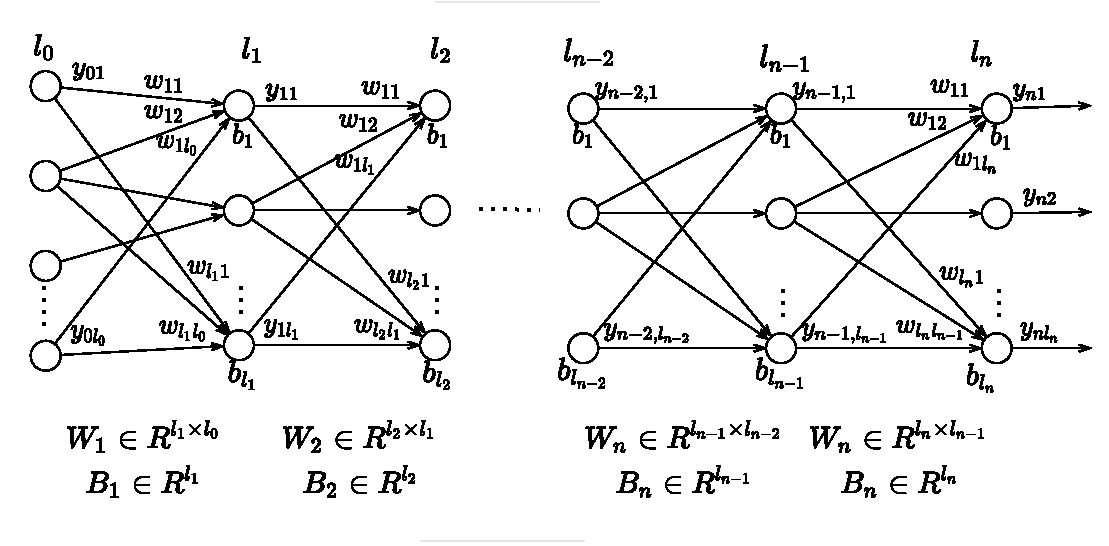
\includegraphics[width=0.9\textwidth]{Figures/NeuralNetworks1.pdf}
  
  El conjunto de pesos $w$ se puede agrupar en un conjunto de $n$ matrices $W=[W_1, W_2, \dots , W_n]$ con los órdenes indicados en la figura. El conjunto de biases se puede agrupar en $n$ vectores $B=[B_1, B_2, \dots, B_n]$. 
\end{frame}

\begin{frame}\frametitle{Backpropagation}
  Para la capa salida, el gradiente  con respecto a cada uno de los pesos $w\in W_n\in\mathbb{R}^{l_n\times l_{n-1}}$ es también una matriz $\nabla y_n \in \mathbb{R}^{l_n\times l_{n-1}}$:
  \[\left[\begin{tabular}{cccc}
      $(y_{n1} - t_1)(y_{n1}-y_{n1}^2)y_{n-1,1}$ & $(y_{n1} - t_1)(y_{n1}-y_{n1}^2)y_{n-1,2}$ & \dots & $(y_{n1} - t_1)(y_{n1}-y_{n1}^2)y_{n-1,l_{n-1}}$ \\
      $(y_{n2} - t_2)(y_{n2}-y_{n2}^2)y_{n-1,2}$ & $(y_{n2} - t_2)(y_{n2}-y_{n2}^2)y_{n-1,2}$ & \dots & $(y_{n1} - t_1)(y_{n1}-y_{n1}^2)y_{n-1,l_{n-1}}$ \\
  \end{tabular}\right]\]
\end{frame}

\begin{frame}\frametitle{Práctica 12 - Redes neuronales}
\end{frame}